\documentclass{llncs}
\usepackage{times}
\usepackage[utf8]{inputenc}

% Comentar para not MAC Users
%\usepackage[applemac]{inputenc}

\usepackage{a4}
%\usepackage[margin=3cm,nohead]{geometry}
\usepackage{epstopdf}
\usepackage{graphicx}
\usepackage{fancyvrb}
\usepackage{amsmath}
\usepackage{enumerate}
%\renewcommand{\baselinestretch}{1.5}

\begin{document}
\mainmatter
\title{Anonimização e Redes Escuras}

\titlerunning{Anonimização e Redes Escuras}

\author{Sérgio Jorge \and João Freitas \and Alexandre Martins}

\authorrunning{Sérgio Jorge \and João Freitas \and Alexandre Martins}

\institute{
University of Minho, Department of  Informatics, 4710-057 Braga, Portugal\\
e-mail: \{a77730,a74814,a77523\}@alunos.uminho.pt
}

\date{1 de outubro de 2018}
\bibliographystyle{splncs}

\maketitle
\begin{abstract}
Quando se fala de anonimização e Dark Web, é natural que se aborde o projeto TOR, o qual nasceu na metade da década de 90 e permite que os utilizadores naveguem na Internet de forma anónima e segura.
\end{abstract}

\section{Introdução} 
\hspace{3mm} Para muitos que usam a Internet, não há nada mais importante do que a anonimidade e a segurança. Cidadãos comuns, ativistas, forças policiais, jornalistas em países de guerra ou em países com regimes opressivos são alguns dos exemplos de pessoas que procuram isso e para estes, existem vários serviços disponíveis que garantem o que procuram. Neste trabalho, vamos nos focar no TOR visto que é o software mais popular dentro do contexto.

\section{A Web}

\hspace{3mm} Na década de 70, a Internet não era mais do que uma rede computadores fechada. Foi desenvolvida e utilizada pelo Departamento de Defesa dos Estados Unidos da América, com fins militares e de pesquisa. Só em 1990 é que a rede se expandiu e o seu uso tornou-se comercial.

\par Hoje em dia, a Internet satisfaz as necessidades de imensas pessoas e entidades, desde empresas a governos, e atualmente estima-se que 4 biliões de pessoas, ou seja, metade da população mundial tem acesso à rede.

\par A Internet pode ser subdividida em três partes:
\begin{enumerate}
\item A Surface Web, que é a parte da internet que pode ser acedida através de motores de busca como Google,Yahoo ou Bing. Em fevereiro de 2017, estimava-se que havia cerca de 1.154 biliões de websites.\cite {Kristin}
\item A Deep Web que consiste em todas as partes da rede a que não se pode aceder através desses motores de busca, como por exemplo, a página dos dados pessoais do portal académico. Estima-se que a Deep Web seja 4 mil a 5 mil vezes maior do que a Surface web.\cite {Kristin}
\item A Dark Web que faz parte da Deep Web, ou seja não pode ser acedida através de motores de busca tradicionais, e só pode ser acedida através de software especial (TOR, I2P, FreeNet, etc). O tamanho da Dark Web é desconhecido.\cite {Kristin}
\end{enumerate}

\begin{figure}
\begin{center}
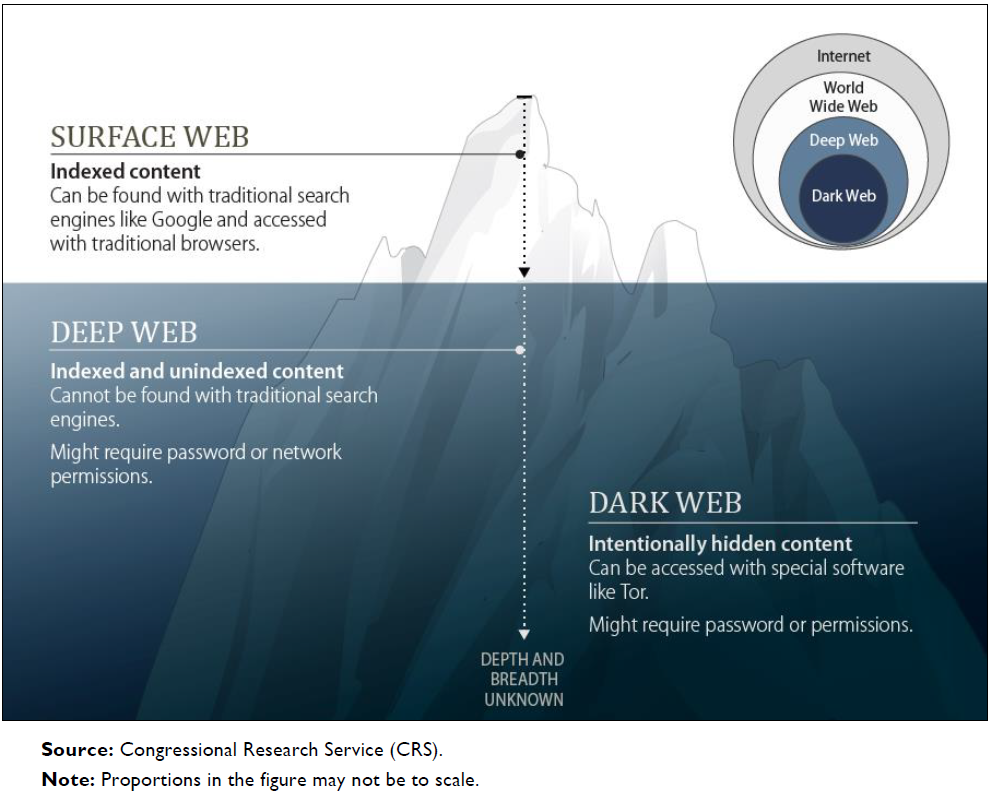
\includegraphics[width=10cm]{Deep.jpg}
\caption{\label{fig:1}As camadas da WEB}
\end{center}
\end{figure}

\pagebreak
\section{TOR}

\subsection{O que é o TOR?}
\hspace{3mm} TOR significa "The Onion Router" e trata-se de um software livre de uso que foi escrito com a finalidade de permitir que os internautas consigam navegar na rede sem serem identificados. Ou seja, idealmente, é possível que as pessoas possam aceder aos diversos sites da Internet sem que ninguém saiba se as pessoas o fizeram realmente. Garante-se, assim, o anonimato e a privacidade ao utilizador.

Os utilizadores vão desde criminosos a forças de segurança, delatores a civis, forças armadas a terroristas. 

\subsection{História do TOR}
\hspace{3mm} O TOR nasceu de um projeto militar, criado pela DARPA (Defense Advanced Research Projects Agency) na década de 90. Inicialmente, foi criado com o intuito de manter o anonimato das forças de segurança. Por exemplo, os agentes infiltrados que precisavam de comunicar com os seus superiores sem serem identificados, ou os oficiais do governo que queriam visitar websites sem que o endereço IP do governo aparecesse nos registos de tráfego. 

\par A partir desta necessidade, Paul Syverson e mais dois matemáticos, criaram o conceito de "onion routing". Basicamente, os pedidos do utilizador iam passando por vários endereços IP na "onion routing network" até chegar ao destino, o que permitia que o utilizador ficasse anónimo. No entanto, o website conseguia ver o último endereço IP que lhe acedeu, e portanto se apenas houvessem pessoas do governo na rede seria fácil de identificar todas as conexões feitas através do TOR como sendo do governo. Isto levou à distribuição do TOR para o público em geral. A segurança e anonimidade da comunicação é diretamente proporcional ao tamanho da rede.

\par Em 2002, com a ajuda de Roger Dingledine e Nick Mathewson, o projeto TOR tornou-se "open-source" e começou a minimizar as ligações com o governo para atrair uma maior audiência.

\par Atualmente, o TOR é mantido por "The TOR Project", que foi fundada em 2006. É uma organização sem fins lucrativos financiada por um grupo de patrocinadores entre eles, agências do governo, utilizadores comuns, corporações e ONGs, como por exemplo a DARPA. Este projeto conta com uma equipa de 60 pessoas sendo que alguns são conhecidos apenas pelos seus nomes de utilizador. \cite{Corianna}

\subsection{Funcionamento do TOR}

\hspace{3mm} As redes de computadores podem-se simplesmente reduzir a uma sequência de sinais elétricos através de cabos de redes, mas é possível, de facto, organizar todo o processo em sete camadas a partir do modelo OSI, em que cada uma é responsável por funções específicas.

\begin{figure}
\begin{center}
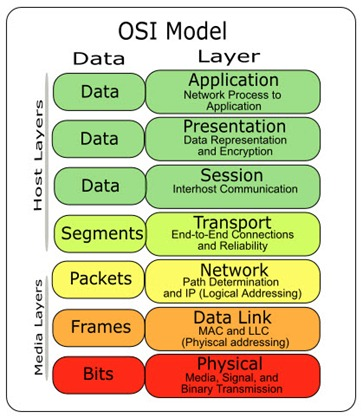
\includegraphics[width=4cm]{osi.jpg}
\caption{\label{fig:2}O modelo OSI}
\end{center}
\end{figure}

\par Na camada de aplicação, a aplicação cliente apresenta a informação ao utilizador e faz o pedido ao servidor através do protocolo HTTP. O formato dos dados a enviar/receber é posteriormente tratado na camada de apresentação. Na camada seguinte, na de sessão, é estabelecida a ligação entre cliente e servidor e na camada de transporte, garante-se a entrega dos pacotes. A camada de rede determina o melhor caminho entre cliente-servidor e na camada de dados, o endereço IP destino é convertido no IP físico da máquina servidor. Por último, na camada física, os cabos ajudam na ligação física entre as máquinas.

\par Portanto, quando se acede a um site comum, o tráfego pode ser rastreado até ao IP origem (a própria máquina que fez o acesso). O que o TOR faz é redirecionar esse tráfego através de uma rede de outros computadores para dificultar o rastreamento dos pacotes, implementando o protocolo SOCKS, que trabalha na camada 5 (sessão) do modelo OSI, para ligar os clientes aos proxies. Assim, obtém-se anonimato em aplicações que usam TCP, sobrepondo camadas de criptografia.
O uso deste protocolo em específico, traz a vantagem da compatibilidade com todas as aplicações que usam conexões Transport Layer Protocol. \cite{Kumm}

\par Usando o TOR Browser como nó de origem, este em vez de comunicar diretamente com o nó de destino, adiciona às mensagens as respetivas chaves criptográficas e faz uma comunicação com um Onion Router ou nó intermédio, que está numa máquina remota. Este, por sua vez, cria também uma conexão com outros nós intermédios até ao destino final. Estabelece-se assim um circuito virtual. \cite{FM}

\pagebreak

\begin{figure}
\begin{center}
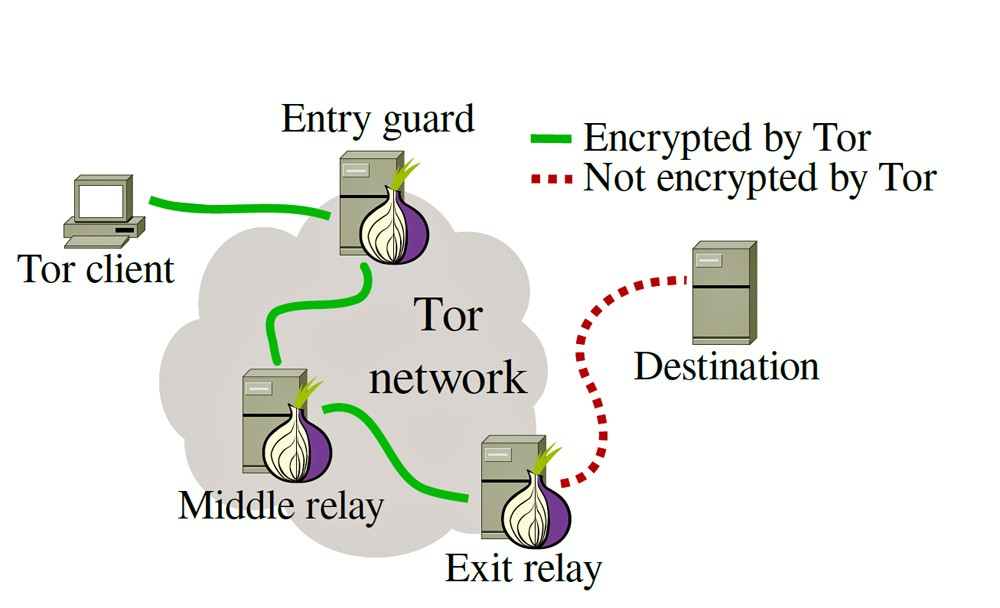
\includegraphics[width=6cm]{tor1.jpg}
\caption{\label{fig:3}A rede TOR}
\end{center}
\end{figure}

\par Ao longo do circuito, cada router só consegue identificar os que lhe são adjacentes (anterior e próximo). Por isso, não é possível rastrear o caminho completo. A cada nó, uma camada de criptografia é descascada revelando o próximo nó para onde o router deve enviar a mensagem. A esta estrutura de dados por camadas damos o nome de Onion já que tudo assemelha-se a uma cebola. \cite{FM}

\begin{figure}
\begin{center}
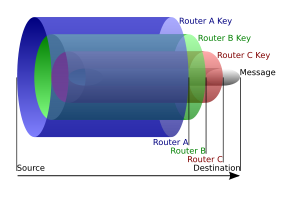
\includegraphics[width=7cm]{tor2.png}
\caption{\label{fig:4}Formato cebola}
\end{center}
\end{figure}

\par Assim, o fluxo de dados é, no mínimo, retransmitido três vezes porque passa necessariamente por um nó de entrada (que apenas sabe o endereço do próximo nó), pelos nós intermédios e pelo nó de saída. 
O nó de saída é o responsável por retirar a criptografia a fim de se conseguir comunicar com o destino final. \cite{Kumm}

\par A lista de todos os nós da rede TOR é pública. Por isso, um país pode bloquear o acesso a estes e impossibilitar que o utilizador consiga ligar-se a um nó de entrada, censurando, assim, o uso da rede anónima. Por isso, foram criados bridges. Tratam-se de nós que não são divulgados ao público. \cite{Kumm}

\par Sem o uso de HTTPS, é possível analisar o tráfego de dados no nó de saída. Por isso, para manter o anonimato, é importante que os diversos sites da rede suportem segurança fim-a-fim.

\subsection{TOR Browser - Como usar?}
\hspace{3mm} Para poder utilizar o serviço TOR, é necessário software específico, como por exemplo o TOR Browser, o mais user-friendly de todos.

Trata-se de um navegador Firefox no qual estão instalados três addons:
 
\begin{enumerate}
\item NoScript que permite desativar o Javascript devido ao perigo de injeções maliciosas de código
\item TorButton que melhora a segurança e facilita a alteração da identidade
\item HTTPS Everywhere que faz com que o navegador use conexões seguras quando disponíveis
\end{enumerate}

Por isso, é simplesmente um Firefox modificado.

\par No entanto, de qualquer das formas, alerta-se para o perigo de abrir ficheiros que foram transferidos através do TOR. Há a possibilidade de serem maliciosos e, se fizerem uma conexão com a rede, esta será feita a partir de uma conexão regular, pelo que a identidade real será revelada.

Para facilitar acesso a sites "escondidos" existem serviços como {$https://thehiddenwiki.org/$} que servem como Google da Dark Web.\cite{Hidden}

\subsection{Será realmente 100\% seguro?}
\hspace{3mm} Apesar de tudo, software como o TOR não é impermeável e várias pessoas foram detidas por causa das operações ilícitas que praticavam na Dark Web. O caso mais sonante foi o de Ross William Ulbricht, dono e criador do website "Silk Road", apelidado "eBay das coisas ilícitas", que servia como mercado de drogas, armas,  cartões de crédito roubados, etc. Ross William Ulbricht foi identificado porque ao pedir ajuda para programar o seu site, forneceu o seu email que continha o nome real. \cite{Ross}

\par Também em 2013, o FBI ganhou controlo do serviço de hospedagem "Freedom Hosting", que hospedava, entre outros, cerca de 40 sites de pornografia infantil. Após ganhar controlo, inseriu um malware neste que enviava o MAC e IP address dos utilizadores, permitindo a subsequente identificação desses. \cite{Free}

\par Todo o tráfego é encriptado do cliente até ao nó de saída. Nesse ponto, se o site não for HTTPS, poderá haver problemas ao nível da deteção da entidade e dos dados. 
\par O TOR não esconde ao ISP o facto de estar a ser utilizado e o ISP sabe que o cliente o está, de facto, a usar mas não sabe para quê.
\par Com isto em mente é recomendado acompanhar o TOR com um VPN visto que é possível fazer backtracking a partir do servidor de destino com objetivo de identificar o utilizador original.

\par Apesar de todas as precauções é quase impossível obter anonimato absoluto, visto que várias táticas foram desenvolvidas para combater software como TOR. Mesmo assim, os serviços secretos americanos dizem que é impossível identificar 100\% dos utilizadores mas é possível de-anonimizar uma fração pequena deles.


"We will never be able to de-anonymize all Tor users all the time but with manual analysis we can de-anonymize a very small fraction of Tor users"
\cite{Ed}

\subsection{Questões morais da rede TOR}
\hspace{3mm} Não há dúvidas que a rede TOR acaba por, apesar de tudo, ser usada como ferramenta para canalizar atitudes e comportamentos das pessoas que, à partida, são censuráveis para a sociedade em geral. É o caso do website WikiLeaks, que mostra documentos importantes com informação confidencial, tais como provas de crimes internacionais ou até textos diplomáticos. Também a transação e a procura por serviços e conteúdos ilegais é comum na rede, pelo que é factual que se vendem drogas ilegais, contratam-se assassinos ou até se partilham conteúdos do mais ilegal que possa existir.

\par No entanto, a rede é também válida para comunicação de jornalistas em países de guerra, para que uma voz num país ditatorial se possa ouvir ou até para expor abusos de guerras civis como a do Afeganistão. Ou seja, todas estas situações de uso da rede são com o propósito da segurança dos utilizadores.

\par Assim, a ferramenta que aqui apresentamos, é mais um meio tecnológico inventado pelo ser humano e, tal como as restantes coisas no mundo, pode ser explorado de formas bem distintas onde nelas se incluem as boas coisas e as más coisas da sociedade. Defende-se assim que a rede TOR e o bem da sociedade não são assim tão inimigos, como alguma da crítica social diz ser.


\section{Conclusões}
\hspace{3mm} Neste trabalho foi aprofundada a anonimização em redes de computadores e a forma como o TOR consegue realizar a tarefa para o qual foi criado. O projeto TOR nasceu e continua a ser financiado pelo governo dos Estados Unidos da América e permite garantir segurança e o anonimato na Internet. Como uma ferramenta, é usada para diversos fins, sejam eles positivos ou não para a sociedade em geral. O que limita o software é precisamente o utilizador que está atrás do monitor e, o anonimato, irá sempre desdobrar-se para o uso legal e moral ou para o uso ilegal e imoral.
\par Hoje em dia, a maioria das nações defende que é importante proteger a identidade das diversas pessoas em prol da segurança e vamos podendo usufruir dele. De qualquer das formas, se não existisse, provavelmente haveria outro método semelhante para o mesmo fim.
\par Constatámos também que o tamanho da Web vai muito para além daquilo que o comum dos mortais julga, já que o tamanho da Dark Web é realmente desconhecido.

\begin{thebibliography}{1}
\bibitem{FM}
Xavier, Fábio.; Silva, Marco.:
\newblock {Deep Web e a Rede Tor: Qual a sua Relação?} (2016)

\bibitem{Kumm}
Kumm, Victor.:
\newblock {Eficácia da utilização da rede TOR para o anonimato e a confidencialidade das comunicações na Internet} (2016)

\bibitem{Corianna}
Jacoby, Corianna.:
\newblock {The Onion Router and the Darkweb}.

\bibitem{Kristin}
Finklea, Kristin.:
\newblock {Dark Web}. (2017)

\bibitem{Hidden}
Wikipedia.:
\newblock {$https://en.wikipedia.org/wiki/The_Hidden_Wiki$}.

\bibitem{Ross}
Ibid.:
\newblock {$https://en.wikipedia.org/wiki/Ross_Ulbricht$}.

\bibitem{Free}
Ibid.:
\newblock {$https://en.wikipedia.org/wiki/Freedom_Hosting$}.

\bibitem{Ed}
NSA,.:
\newblock {$https://edwardsnowden.com/docs/doc/tor-stinks-presentation.pdf$} (Tor Stinks).

\end{thebibliography}

\end{document}